%% FullCourse_10Lecs -- Lecture 9, Topic 9.6: Lec10 Preview + Wrap-up + Appendix
%% Source: ./archive_pre_split/Lec09_Agentic_AI_v3.tex (sections 12-14)
%% Pass B: layer in refinements from
%%         ../../MiniCourse_8hr/Slides/Module4_Agentic_AI/M4_T10_Wrapup_Research_Judgment.tex

%% Shared preamble for the FullCourse_10Lecs topic decks.
%%
%% Each topic .tex \input's this file, then defines its own \title, \date
%% override (if any), \graphicspath, and \begin{document}.
%%
%% Reconstructed verbatim from the inlined copy preserved in
%% Lec10_Case_Studies/Lec10_T8_Case6_DeepRamsey.tex (lines 23-190), which is
%% explicitly annotated there as "from ../shared_preamble.tex, copied verbatim".
%% Base preamble matches MiniCourse_8hr/Slides/shared_preamble.tex; this version
%% additionally provides \sectiondivider, the conceptbox/cautionbox/examplebox/
%% takeawaybox tcolorboxes, and \compacttables used across the split decks.

\documentclass[10pt,english,aspectratio=169]{beamer}

\usepackage{ae,aecompl}
\usepackage[T1]{fontenc}
\usepackage{textcomp}
\usepackage[utf8]{inputenc}
\usepackage{babel}
\usepackage{datetime2}

\setcounter{secnumdepth}{3}
\setcounter{tocdepth}{3}

\usepackage{amsmath, amssymb, amsthm, graphicx}
\usepackage{booktabs, multirow}
\usepackage{tikz}
\usepackage{pgfplots}
\pgfplotsset{compat=1.16}
\usepackage[most]{tcolorbox}
\tcbuselibrary{skins, breakable, theorems}
\usepackage{listings}
\usepackage{xcolor}

\lstset{
  basicstyle=\ttfamily\small,
  keywordstyle=\color{blue!80!black}\bfseries,
  commentstyle=\color{green!50!black}\itshape,
  stringstyle=\color{orange!80!black},
  backgroundcolor=\color{gray!8},
  frame=single,
  rulecolor=\color{gray!40},
  breaklines=true,
  showstringspaces=false,
  numbers=none,
}

\lstdefinestyle{pythonstyle}{
    language=Python,
    basicstyle=\ttfamily\footnotesize,
    keywordstyle=\color{blue!80!black}\bfseries,
    commentstyle=\color{green!50!black}\itshape,
    stringstyle=\color{orange!80!black},
    frame=single,
    breaklines=true,
    showstringspaces=false,
    numbers=left,
    numbersep=5pt,
    numberstyle=\tiny\color{gray},
    backgroundcolor=\color{gray!8},
    rulecolor=\color{gray!40}
}

\ifx\hypersetup\undefined
  \AtBeginDocument{%
    \hypersetup{bookmarks=false,breaklinks=true,pdfborder={0 0 0},colorlinks=true,
      linkcolor=DarkText,urlcolor=RedTitle}%
  }
\else
  \hypersetup{bookmarks=false,breaklinks=true,pdfborder={0 0 0},colorlinks=true,
    linkcolor=DarkText,urlcolor=RedTitle}%
\fi

\makeatletter
\newcommand\makebeamertitle{%
  \begin{frame}[plain]
    \vspace*{1.0cm}
    \centering
    {\usebeamerfont{title}\usebeamercolor[fg]{title}\inserttitle\par}
    \vspace{1.0cm}
    {\usebeamerfont{author}\usebeamercolor[fg]{author}\insertauthor\par}
    \vspace{0.2cm}
    {\usebeamerfont{date}\usebeamercolor[fg]{date}\insertdate\par}
  \end{frame}}%
\AtBeginDocument{%
  \let\origtableofcontents=\tableofcontents
  \def\tableofcontents{\@ifnextchar[{\origtableofcontents}{\gobbletableofcontents}}
  \def\gobbletableofcontents#1{\origtableofcontents}%
}

\usetheme{metropolis}
\usefonttheme{professionalfonts}

\definecolor{LightGray}{RGB}{230,230,230}
\definecolor{RedTitle}{RGB}{0,0,200}
\definecolor{VeryLightGray}{RGB}{245,245,245}
\definecolor{DarkText}{RGB}{0,0,0}

\setbeamercolor{background canvas}{bg=white}
\setbeamercolor{title}{fg=RedTitle}
\setbeamercolor{author}{fg=DarkText}
\setbeamercolor{date}{fg=DarkText}
\setbeamercolor{frametitle}{bg=VeryLightGray,fg=DarkText}
\setbeamercolor{normal text}{fg=DarkText}
\setbeamerfont{title}{size=\large}

\setbeamersize{text margin left=5mm, text margin right=5mm}
\addtobeamertemplate{frametitle}{}{\vspace{-0.5em}}
\newcommand{\reducevspace}{\vspace{-0.5cm}}

% Shared section divider and box styles for split topic decks.
\newcommand{\sectiondivider}[2]{%
\begin{frame}[plain,noframenumbering]
\begin{center}
\vfill
{\Large\textbf{#1}\par}
\vspace{0.35cm}
{\normalsize #2\par}
\vfill
\end{center}
\end{frame}
}

\newtcolorbox{conceptbox}[1][]{
  colback=blue!3,
  colframe=RedTitle!55,
  boxrule=0.35mm,
  arc=1mm,
  left=2mm,
  right=2mm,
  top=1mm,
  bottom=1mm,
  #1
}
\newtcolorbox{cautionbox}[1][]{
  colback=red!3,
  colframe=red!50!black,
  boxrule=0.35mm,
  arc=1mm,
  left=2mm,
  right=2mm,
  top=1mm,
  bottom=1mm,
  #1
}
\newtcolorbox{examplebox}[1][]{
  colback=green!3,
  colframe=green!45!black,
  boxrule=0.35mm,
  arc=1mm,
  left=2mm,
  right=2mm,
  top=1mm,
  bottom=1mm,
  #1
}
\newtcolorbox{takeawaybox}[1][]{
  colback=VeryLightGray,
  colframe=RedTitle!55,
  boxrule=0.35mm,
  arc=1mm,
  left=2mm,
  right=2mm,
  top=1mm,
  bottom=1mm,
  #1
}
\newcommand{\compacttables}{\renewcommand{\arraystretch}{1.15}}

\setbeamertemplate{navigation symbols}{}
\setbeamertemplate{footline}{%
  \hfill%
  \usebeamercolor[fg]{page number in head/foot}%
  \usebeamerfont{page number in head/foot}%
  \insertframenumber\,/\,\inserttotalframenumber\kern1em\vskip2pt%
}

\makeatother

\author{Zhigang Feng}
% "date with time": compile timestamp so each build is identifiable.
\date{\today\ \DTMcurrenttime}


% Suppress redundant auto-generated metropolis section page; \sectiondivider frames are the dividers we keep.
\metroset{sectionpage=none}

\graphicspath{{./pic/}{./figures/}{../../MiniCourse_8hr/Slides/Module4_Agentic_AI/pic/}{../}}


\usetikzlibrary{positioning,arrows.meta,shapes,calc}

\title[AI for Econ Research]{AI for Economic Research: Dynamic Models, Language, and Agents\\
Lecture 9.6: Lecture 10 Preview, Wrap-up, and Appendix}

\begin{document}

\makebeamertitle

%=============================================================================
\begin{frame}{Topic 9.6 Agenda}
\begin{enumerate}
  \item \textbf{Lecture 10 Preview} --- case studies on the horizon
  \medskip
  \item \textbf{Three Econometric Roles} --- signal, outcome, instrument
  \medskip
  \item \textbf{Wrap-up} --- six criteria, when not to use an agent, what stays human
  \medskip
  \item \textbf{Appendix}
\end{enumerate}

\bigskip
\footnotesize\textit{Arc: T1 Framing $\to$ T2 Under the Hood $\to$ T3 Homotopy $\to$ T4 Project Org $\to$ T5 Mistakes/Context $\to$ \textbf{T6 Wrap.}}
\end{frame}

%=============================================================================
\section{Lecture 10 Preview: Case Studies}
%===========================================================

\sectiondivider{Lecture 10 Preview}{From workflow logic to concrete case studies}

\begin{frame}{Lecture 10 Preview: Four Concrete Workflow Patterns}
\begin{center}
\small
\begin{tabular}{|p{2.7cm}|p{3.7cm}|p{4.7cm}|}
\hline
\textbf{Pattern} & \textbf{Lecture 10 case} & \textbf{What students will see} \\ \hline
Reusable skill & Paper-review workflow & staged quality control, quote checks, editorial filter \\ \hline
Empirical pipeline & MEPS uninsurance & harmonization, survey weights, benchmark validation, figures \\ \hline
Public-web dataset & Fellows metadata & source restrictions, provenance, missingness discipline \\ \hline
Full-lifecycle collaborator & Glue-work research project & theory, pipeline design, critique, claims discipline \\ \hline
\end{tabular}
\end{center}

\vspace{0.25cm}
\textbf{Why this matters:} Lec.~9 gives the workflow logic. Lec.~10 shows how the same logic changes shape across different research artifacts.
\end{frame}

\begin{frame}{One Visual Hook from Lecture 10: MEPS Uninsurance}
\textbf{Case Study 2 asks:} who is uninsured in the United States, 2000--2023, and how did the ACA change the distribution?

\vspace{0.25cm}

\begin{center}
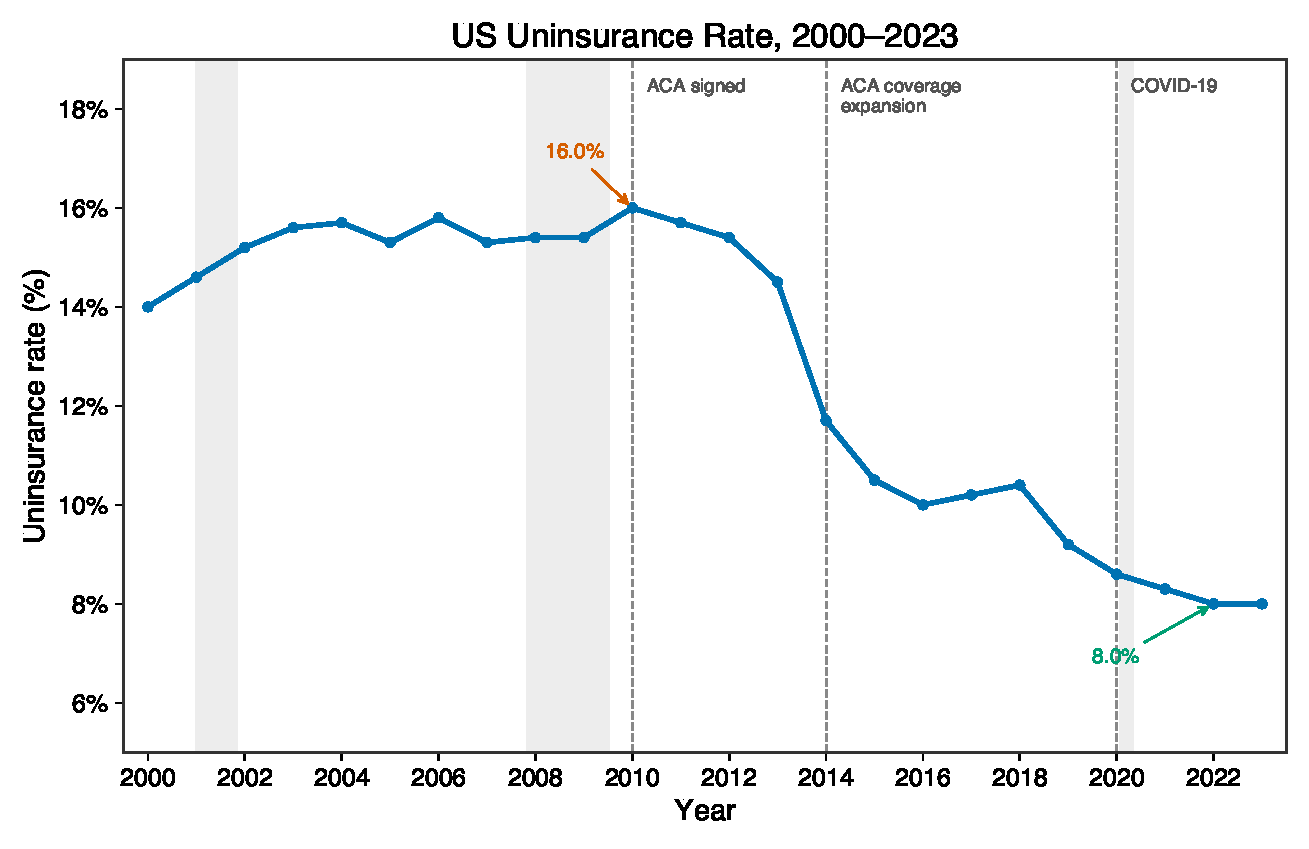
\includegraphics[height=0.38\textheight]{fig_overall_uninsurance.pdf}
\end{center}

\textbf{Why keep this figure here:} it is an accessible policy example for economists outside macro, and it shows what a validated empirical artifact looks like after the workflow succeeds.

\vspace{0.15cm}

\textbf{Lec.~10 adds the full pipeline:} prompts, schema harmonization, survey weights, external benchmarks, and subgroup figures.
\end{frame}

\begin{frame}{Three Econometric Roles in Agent-Assisted Research}
\textbf{Lec07 T4 introduced a taxonomy: every text-derived variable plays one of three roles --- \emph{signal}, \emph{outcome}, or \emph{instrument}. The four Lec10 patterns get sharper when we apply that lens.}

\vspace{0.18cm}

\begin{center}
\footnotesize
\renewcommand{\arraystretch}{1.15}
\begin{tabular}{|p{2.7cm}|p{2.4cm}|p{2.6cm}|p{3.4cm}|}
\hline
\textbf{Pattern} & \textbf{Signal} & \textbf{Outcome} & \textbf{Instrument} \\ \hline
Reusable skill (paper review) & methodological rigor & review quality & staged evaluation rubric \\ \hline
Empirical pipeline (MEPS) & uninsurance rates & health-coverage estimates & survey-weighted harmonization \\ \hline
Public-web dataset (fellows) & field assignment & provenance log & source-restriction rules \\ \hline
Full-lifecycle collaborator (glue-work) & research idea & validated claims & agent $+$ domain expert critique \\ \hline
\end{tabular}
\end{center}

\vspace{0.12cm}
\textbf{Same agent toolkit, four research designs.} The taxonomy makes you ask: what role does the agent's output play in your inference?
\end{frame}

\begin{frame}{What to Watch for in Lecture 10}
\begin{itemize}
    \item \textbf{Paper review:} how a reusable skill turns a vague prompt into a staged quality-control workflow
    \item \textbf{MEPS pipeline:} how an empirical question becomes a validated panel and figure set
    \item \textbf{Fellows dataset:} how provenance and missingness rules matter as much as code
    \item \textbf{Glue-work project:} how agentic AI can act as a full-lifecycle collaborator without replacing human claims discipline
\end{itemize}

\vspace{0.3cm}
\textbf{Bridge from Lec.~9 to Lec.~10:} today's lecture explains the logic of the workflow; next lecture shows the artifacts it can produce.
\end{frame}

%===========================================================
%=============================================================================
\section{Wrap-up}
%===========================================================

\sectiondivider{Wrap-up}{What the workflow changes and what remains human}

% MiniCourse refinement: research judgment framing from M4_T10
\begin{frame}{Six Criteria for Any AI-Assisted Research Output}
\textbf{Before accepting a script, figure, or table the agent produced, run it past six questions.}

\vspace{0.18cm}

\begin{center}
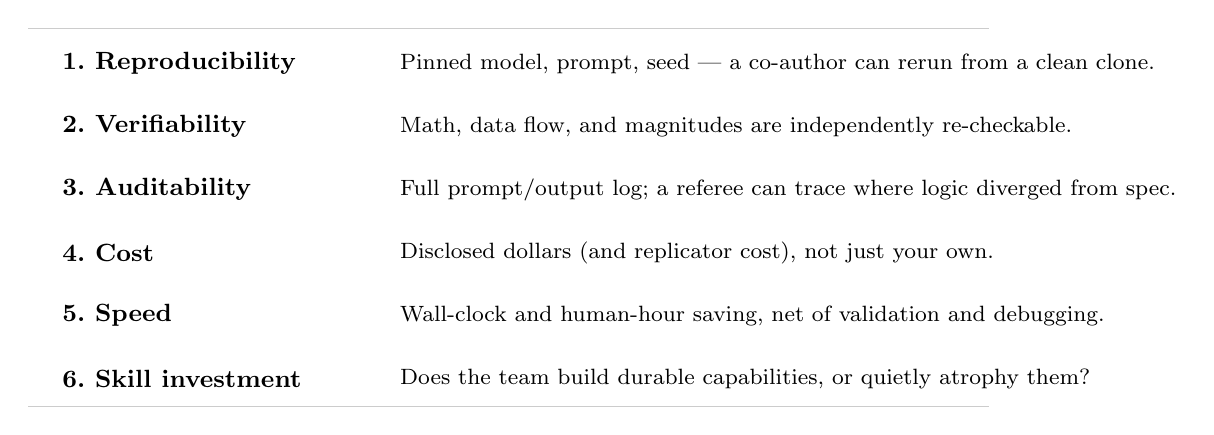
\begin{tikzpicture}
    \node[anchor=west, font=\small] at (0, 4.0) {$\square$ \textbf{1.\ Reproducibility}};
    \node[anchor=west, font=\footnotesize] at (4.4, 4.0) {Pinned model, prompt, seed --- a co-author can rerun from a clean clone.};

    \node[anchor=west, font=\small] at (0, 3.2) {$\square$ \textbf{2.\ Verifiability}};
    \node[anchor=west, font=\footnotesize] at (4.4, 3.2) {Math, data flow, and magnitudes are independently re-checkable.};

    \node[anchor=west, font=\small] at (0, 2.4) {$\square$ \textbf{3.\ Auditability}};
    \node[anchor=west, font=\footnotesize] at (4.4, 2.4) {Full prompt/output log; a referee can trace where logic diverged from spec.};

    \node[anchor=west, font=\small] at (0, 1.6) {$\square$ \textbf{4.\ Cost}};
    \node[anchor=west, font=\footnotesize] at (4.4, 1.6) {Disclosed dollars (and replicator cost), not just your own.};

    \node[anchor=west, font=\small] at (0, 0.8) {$\square$ \textbf{5.\ Speed}};
    \node[anchor=west, font=\footnotesize] at (4.4, 0.8) {Wall-clock and human-hour saving, net of validation and debugging.};

    \node[anchor=west, font=\small] at (0, 0.0) {$\square$ \textbf{6.\ Skill investment}};
    \node[anchor=west, font=\footnotesize] at (4.4, 0.0) {Does the team build durable capabilities, or quietly atrophy them?};

    \draw[gray!40] (-0.2, 4.45) -- (12, 4.45);
    \draw[gray!40] (-0.2, -0.35) -- (12, -0.35);
\end{tikzpicture}
\end{center}

\vspace{0.1cm}
\begin{center}
\textit{If any answer is ``no'' or ``I don't know,'' the artifact is not yet research-grade.}
\end{center}
\end{frame}

\begin{frame}{Three Things AI Cannot Do --- Regardless of Capability}
\small
\begin{itemize}
  \item \textbf{Identification.} \\
  Choosing the variation that answers the causal question. \\
  An LLM does not know which shock is exogenous, which instrument is valid, or which event window is contaminated. It can describe identification strategies; it cannot \emph{certify} one for your setting.

  \vspace{0.1cm}
  \item \textbf{Welfare.} \\
  Choosing the objective function that defines ``good.'' \\
  Pareto weights, planner discount rates, equity--efficiency trade-offs --- these are normative choices the researcher must own.

  \vspace{0.1cm}
  \item \textbf{Judgment.} \\
  Choosing which question is worth asking. \\
  AI optimizes against a stated target; only economists decide which target is interesting, novel, and policy-relevant.
\end{itemize}

\vspace{0.15cm}
\begin{center}
\textit{These are not gaps that scale away with model size --- they are categorically outside the system.}
\end{center}
\end{frame}

\begin{frame}{When NOT to Use an Agent}
\textbf{The six criteria can also serve as a boundary: there are research tasks where the agent overhead exceeds the benefit, or where the failure mode is too costly.}

\vspace{0.2cm}

\begin{itemize}
    \item \textbf{One-line scripts and isolated edits.} A two-line \texttt{sed} or one-shot plot has no validation surface for the harness to add value. Open the editor.
    \item \textbf{Deeply proprietary or undocumented pipelines.} If the conventions live in one person's head, the agent has nothing to read; the time you would spend documenting the pipeline well enough to brief the agent is the same time you would spend just fixing the thing.
    \item \textbf{Strict deterministic guarantees.} For numerical reproducibility audits, regulatory pipelines, or replication packages, model nondeterminism is a hazard the harness cannot fully suppress. Run it pinned; do not let the agent retry.
    \item \textbf{Restricted-data analyses where prompts may leak.} If pasting one column would violate IRB or HIPAA, the agent does not belong in the loop; T5's security workarounds apply.
    \item \textbf{Tasks where you do not yet have a benchmark.} Without a way to validate, faster output just means faster wrong. Define the V0 benchmark first; \emph{then} bring in the agent.
\end{itemize}

\vspace{0.1cm}
\footnotesize\textbf{Practical rule:} the agent is most useful when the work is bounded, validated, and repeatable. None of those? Skip the agent.
\end{frame}

\begin{frame}{Trust but Verify}
\begin{enumerate}
    \item Reproduce one statistic by hand
    \item Cross-check one result with another package or script
    \item Test a limiting case or zero-variance benchmark
    \item Read the code line by line where the economics enters
    \item Ask whether the magnitude and sign make sense
\end{enumerate}

\vspace{0.3cm}

\textbf{This is not optional ceremony.} It is what turns fast code into defensible research.
\end{frame}

\begin{frame}{What Changes for Economic Research}
\begin{itemize}
    \item The distance from question to first result shrinks
    \item More specifications become cheap enough to try
    \item Reproducibility can improve because workflow is written down
    \item The premium shifts away from typing speed and toward design, judgment, and validation
\end{itemize}

\vspace{0.3cm}

\textbf{What stays human:} asking the question, choosing the design, knowing the data, and interpreting the output.
\end{frame}

\begin{frame}{You Are the Research Architect}
\begin{center}
\Large
Agents can lay bricks quickly.\\
\textbf{You still design the structure.}
\end{center}

\vspace{0.35cm}

\begin{itemize}
    \item Weak specification produces wrong models
    \item Weak algorithm choice produces slow or misleading computation
    \item Weak numerical judgment produces fragile results
    \item Weak code literacy produces unverified output
\end{itemize}

\vspace{0.25cm}

\textbf{The lecture is not about surrendering expertise.} It is about reallocating effort toward the parts of research that remain scarce.
\end{frame}

\begin{frame}{First Exercise and Looking Ahead}
\textbf{Best first exercise:} take one old project and ask an agent to help clean it up safely.

\vspace{0.25cm}

\begin{itemize}
    \item put the project under Git
    \item create a simple \texttt{CLAUDE.md}
    \item identify one repeated workflow worth encoding
    \item rerun the cleaned project and compare outputs
\end{itemize}

\vspace{0.3cm}

\textbf{Lec.~10:} we return to case studies and let students run a full workflow themselves.

\vspace{0.15cm}

\textit{If you want setup details for the lab, see the appendix.}
\end{frame}

%===========================================================
% TODO Pass B: layer in M4_T10_Wrapup_Research_Judgment refinements

%=============================================================================
\section{Appendix}
%===========================================================

\sectiondivider{Appendix}{Setup notes and dated product details}

\begin{frame}[fragile]{Appendix A: Installing One Terminal Agent (Dated)}
\textbf{Three operational steps, illustrated with Claude Code on macOS:}

\vspace{0.1cm}
\begin{enumerate}
    \item \textbf{Install the runtime} (Node.js for Claude Code; Python for Aider; analogous for others):
\begin{lstlisting}[style=pythonstyle,language={},basicstyle=\ttfamily\tiny,numbers=none]
brew install node  # or download from nodejs.org (v18+)
\end{lstlisting}
    \item \textbf{Install the agent CLI:}
\begin{lstlisting}[style=pythonstyle,language={},basicstyle=\ttfamily\tiny,numbers=none]
npm install -g @anthropic-ai/claude-code   # Claude Code
# pip install codex-cli                    # OpenAI Codex CLI
# pip install aider-chat                   # Aider
\end{lstlisting}
    \item \textbf{Verify:} \texttt{claude --version}, then \texttt{cd your-project-folder \&\& claude}.
\end{enumerate}

\vspace{0.1cm}
\footnotesize\textbf{Mac + OneDrive note:} always \texttt{cd} into the project folder before launching the agent. Running from a \texttt{/Volumes/\ldots} path can trigger permission errors.

\vspace{0.05cm}
\textbf{Dated note:} subscription tiers, model IDs, and install commands change every few months. Recheck the official docs before teaching or running the lab.
\end{frame}

\begin{frame}{Appendix A2: Setup for the Lab}
\textbf{Lightweight setup checklist for a terminal-agent workflow}

\vspace{0.2cm}

\begin{itemize}
    \item Install one terminal agent and confirm it launches
    \item Create a project folder with a project-specific system prompt (e.g., \texttt{CLAUDE.md}, \texttt{AGENTS.md}, \texttt{GEMINI.md}), \texttt{scripts/}, and \texttt{output/}
    \item Make sure Python or R runs from the terminal
    \item Keep the first session small: one file, one check, one output
\end{itemize}

\vspace{0.25cm}

\textbf{Dated note:} exact setup steps, plans, and rate limits change quickly. Recheck the official docs before the lab.
\end{frame}

\begin{frame}[fragile]{Appendix B: Keybindings and Minimal Templates}
\begin{columns}[T]
\begin{column}{0.48\textwidth}
\textbf{Useful commands}

\vspace{0.15cm}
\footnotesize
\begin{tabular}{|l|l|}
\hline
Compact session & \texttt{/compact} \\ \hline
Clear session & \texttt{/clear} \\ \hline
Interrupt & \texttt{Esc} \\ \hline
Slash menu & \texttt{/} \\ \hline
\end{tabular}
\end{column}
\begin{column}{0.48\textwidth}
\textbf{Minimal project-system-prompt}
\begin{lstlisting}[style=pythonstyle,language={},basicstyle=\ttfamily\tiny,numbers=none]
# CLAUDE.md / AGENTS.md / GEMINI.md
Project: ...
Goal: ...
Language: ...
Checks: ...
\end{lstlisting}
\end{column}
\end{columns}
\end{frame}

\begin{frame}{Appendix C: Dated Comparisons and Resources}
\textbf{As of April 2026, examples of terminal-agent workflows include:}
\begin{itemize}
    \item Claude Code
    \item Codex CLI
    \item Gemini CLI
    \item Aider
\end{itemize}

\vspace{0.25cm}

\textbf{Good places to recheck before teaching:}
\begin{itemize}
    \item official Claude Code documentation
    \item official OpenAI Codex CLI documentation
    \item course notes and lab instructions
\end{itemize}

\vspace{0.2cm}

\textbf{Teaching rule:} keep dated product comparisons in the appendix, not in the conceptual core of the lecture.
\end{frame}

\begin{frame}{Appendix D: Context Dilemma --- References}
\scriptsize

\textbf{Context as implicit prior}
\begin{itemize}
    \item Xie, Raghunathan, Liang, Ma (2022). An Explanation of In-context Learning as Implicit Bayesian Inference. ICLR. arXiv:2111.02080.
\end{itemize}

\textbf{Sycophancy and RLHF limits}
\begin{itemize}
    \item Sharma et al.\ (2023). Towards Understanding Sycophancy in Language Models. arXiv:2310.13548.
    \item Perez et al.\ (2023). Discovering Language Model Behaviors with Model-Written Evaluations. ACL Findings. arXiv:2212.09251.
    \item Casper et al.\ (2023). Open Problems and Fundamental Limitations of RLHF. TMLR. arXiv:2307.15217.
    \item Wolf et al.\ (2023). Fundamental Limitations of Alignment in Large Language Models. arXiv:2304.11082.
\end{itemize}

\textbf{Self-correction and adversarial review}
\begin{itemize}
    \item Huang et al.\ (2024). Large Language Models Cannot Self-Correct Reasoning Yet. ICLR. arXiv:2310.01798.
    \item Valmeekam et al.\ (2023). Can Large Language Models Really Improve by Self-critiquing Their Own Plans? NeurIPS. arXiv:2310.08118.
    \item Du et al.\ (2023). Improving Factuality and Reasoning through Multiagent Debate. arXiv:2305.14325.
    \item Irving, Christiano, Amodei (2018). AI Safety via Debate. arXiv:1805.00899.
\end{itemize}

\textbf{Monoculture and the economist workflow}
\begin{itemize}
    \item Kleinberg \& Raghavan (2021). Algorithmic Monoculture and Social Welfare. PNAS 118(22).
    \item Bommasani et al.\ (2022). Picking on the Same Person: Does Algorithmic Monoculture Lead to Outcome Homogenization? NeurIPS. arXiv:2211.13972.
    \item Korinek (2023). Language Models and Cognitive Automation for Economic Research. NBER WP 30957; JEL.
\end{itemize}
\end{frame}

\end{document}
